\documentclass[12pt,a4paper]{article}
\usepackage[utf8]{inputenc}
\usepackage[T1]{fontenc}
\usepackage[french]{babel}
\usepackage{geometry}
\usepackage{xcolor}
\usepackage{listings}
\usepackage{graphicx}
\usepackage{titlesec}
\usepackage{hyperref}


\geometry{margin=2.5cm}
\definecolor{codegreen}{rgb}{0,0.6,0}
\definecolor{codegray}{rgb}{0.5,0.5,0.5}
\definecolor{codepurple}{rgb}{0.58,0,0.82}
\definecolor{backcolour}{rgb}{0.95,0.95,0.92}

\lstdefinestyle{plsql}{
    backgroundcolor=\color{backcolour},
    commentstyle=\color{codegreen},
    keywordstyle=\color{magenta},
    numberstyle=\tiny\color{codegray},
    stringstyle=\color{codepurple},
    basicstyle=\ttfamily\footnotesize,
    breakatwhitespace=false,
    breaklines=true,
    captionpos=b,
    keepspaces=true,
    numbers=left,
    numbersep=5pt,
    showspaces=false,
    showstringspaces=false,
    showtabs=false,
    tabsize=4,
    frame=single,
    language=SQL
}

\titleformat{\section}{\large\bfseries}{\thesection}{1em}{}[{\titlerule[0.8pt]}]

\title{TP PL/SQL -  schéma HR}
\author{Lyes Rahal }
\date{\today}
\vspace{1cm}


\begin{document}

\maketitle
\noindent\textbf{Lien GitHub du projet :} \\
\url{https://github.com/Rahal-Lyes/plsql-cursor}

\tableofcontents
\newpage
\section{Partie A : Affichage des informations des employés}
\subsection{Version avec curseur explicite}
\begin{lstlisting}[style=plsql]
DECLARE
    CURSOR c_emp IS 
        SELECT E.FIRST_NAME, J.JOB_TITLE, J.MAX_SALARY
        FROM EMPLOYEES E
        JOIN JOBS J ON E.JOB_ID = J.JOB_ID;
    v_emp_rec c_emp%ROWTYPE;
    
BEGIN
    OPEN c_emp;
    LOOP
        FETCH c_emp INTO v_emp_rec;
        EXIT WHEN c_emp%NOTFOUND;
        DBMS_OUTPUT.put_line(v_emp_rec.first_name|| ' est un ' || v_emp_rec.JOB_TITLE|| ' il touch u salaire  de ******' ||v_emp_rec.MAX_SALARY);
    END LOOP;
    CLOSE c_emp;
END;
/\end{lstlisting}

\subsection{Autre method ameliorer pour la question A}
\begin{lstlisting}[style=plsql]
DECLARE
    CURSOR c_emp IS 
        SELECT E.FIRST_NAME, J.JOB_TITLE, J.MAX_SALARY
        FROM EMPLOYEES E
        JOIN JOBS J ON E.JOB_ID = J.JOB_ID
        ORDER BY E.FIRST_NAME;
BEGIN
  FOR v_emp_rec IN c_emp LOOP
    DBMS_OUTPUT.put_line(v_emp_rec.first_name|| ' est un ' || v_emp_rec.JOB_TITLE|| ' il touch u salaire  de ****' ||v_emp_rec.MAX_SALARY);
    END LOOP;
    DBMS_OUTPUT.PUT_LINE(v_separator);
END;
/\end{lstlisting}
\newpage
\section{Partie B : Fonction de calcul de salaire}
\begin{lstlisting}[style=plsql]
  CREATE OR REPLACE FUNCTION new_sal (
    old_sal IN NUMBER,
    pct     IN NUMBER
 ) RETURN NUMBER 
 AS
    new_salary EMPLOYEES.salary%TYPE;
    pct_null_exc EXCEPTION;
 BEGIN
    IF pct IS NOT NULL THEN
       new_salary := old_sal * (1 + pct);
       RETURN new_salary;
    ELSE
       RAISE pct_null_exc;
    END IF;
 
 EXCEPTION
    WHEN pct_null_exc THEN
       DBMS_OUTPUT.PUT_LINE('La valeur de pct de l''employé est NULL');
       RETURN NULL;  
 END;
/\end{lstlisting}
\newpage
\section{Partie C : Ajout de l’attribut \texttt{new\_salary} de type \texttt{NUMBER} à la table \texttt{EMPLOYEES}}

\begin{lstlisting}[style=plsql]
  ALTER TABLE EMPLOYEES ADD new_salary  NUMBER(8,2);
\end{lstlisting}

\section{Partie D : Procédure de mise à jour}
\begin{lstlisting}[style=plsql]
  CREATE OR REPLACE PROCEDURE new_salary AS 
  CURSOR emp_cursor IS
    SELECT employee_id, salary, commission_pct
    FROM EMPLOYEES;
    

  new_sal_value EMPLOYEES.salary%TYPE;

BEGIN
  
  FOR i IN emp_cursor LOOP
    new_sal_value := new_sal(i.salary, i.commission_pct);
    UPDATE EMPLOYEES
    SET new_salary = new_sal_value
    WHERE employee_id = i.employee_id;
  END LOOP;

  COMMIT; 
END;
/\end{lstlisting}
\section{Partie E: Exécuter la procédure et montrer les résultats de son exécution (avant et après)}
\begin{figure}[h!]
  \centering
  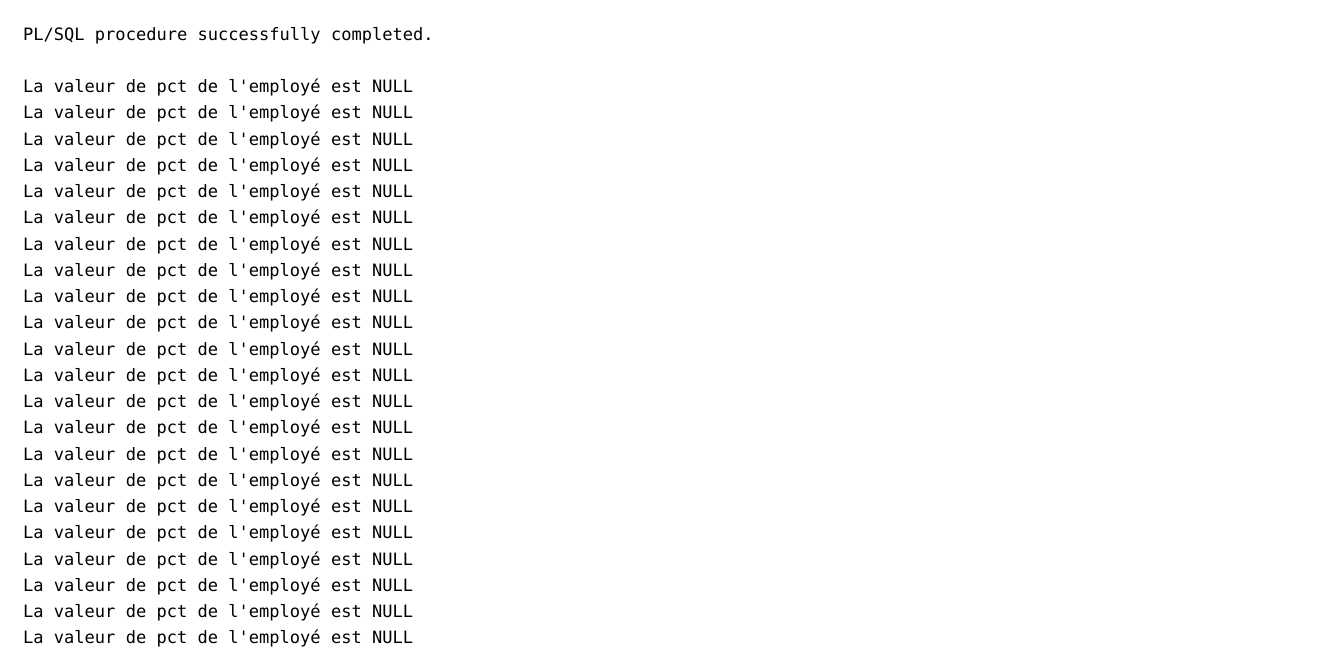
\includegraphics[width=0.7\textwidth]{01.png}
  \caption{L'exécution de la procédure new_salary}
  \label{fig:mon_image}
\end{figure}
\newpage
\section{Partie F: Afficher les informations sur les old et new salary sous cette forme)}

\begin{lstlisting}[style=plsql]
  DECLARE
  CURSOR c_emp is SELECT E.FIRST_NAME,E.SALARY,E.NEW_SALARY
  FROM EMPLOYEES E;
  v_emp_rec c_emp %rowtype;
  
  BEGIN
    OPEN c_emp;
    LOOP
     FETCH c_emp into v_emp_rec;
     exit when c_emp %notfound;
  
     DBMS_OUTPUT.put_line(v_emp_rec.first_name|| '      ,ancien salaire *****' || v_emp_rec.SALARY|| '       nouveau salaire  ******' ||v_emp_rec.NEW_SALARY);
     END LOOP;
     CLOSE c_emp;
  
    END;
    /
  \end{lstlisting}
\newpage
  \section{(g) Programme PL/SQL utilisant un curseur}

  Le programme suivant utilise un curseur pour afficher les informations suivantes pour chaque employé :
  \begin{itemize}
    \item Nom de l'employé
    \item Son poste (job)
    \item La date de début d’emploi
    \item L’expérience exprimée en nombre de jours (arrondi sans virgule)
    \item L’expérience exprimée en nombre de mois (arrondi sans virgule)
  \end{itemize}
  

  \begin{lstlisting}[style=plsql]
  
DECLARE 
CURSOR c_employe IS SELECT E.FIRST_NAME,J.JOB_TITLE,JH.START_DATE,JH.END_DATE
FROM EMPLOYEES E
JOIN JOBS J ON j.JOB_ID=E.JOB_ID
JOIN JOB_HISTORY JH ON JH.JOB_ID=J.JOB_ID;


v_nom EMPLOYEES.FIRST_NAME %type;
v_job_title JOBS.JOB_TITLE %type;
v_start_date JOB_HISTORY.START_DATE%type;
v_end_date JOB_HISTORY.END_DATE%type;
v_experience_jours NUMBER;
v_experience_mois  NUMBER;
v_emp_rec c_employe%rowtype;
BEGIN
  OPEN c_employe;
  LOOP
    FETCH c_employe into v_emp_rec;
    exit when c_employe%notfound;
    v_nom :=v_emp_rec.FIRST_NAME;
    v_job_title :=v_emp_rec.JOB_TITLE;
    v_start_date :=v_emp_rec.START_DATE;
    v_end_date := v_emp_rec.END_DATE;
  v_experience_jours := TRUNC(v_end_date - v_start_date);
  v_experience_mois  := ROUND(MONTHS_BETWEEN(v_end_date, v_start_date));
    dbms_output.PUT_LINE('Nom_employer '|| v_nom|| '| Son job '||v_job_title|| '| Date_debut d’emploi ' 
    ||v_start_date||'| Expérience en jours '||v_experience_jours ||' Jours'|| '| Expérience en mois '|| v_experience_mois || ' mois');
    end loop;
    CLOSE c_employe;


END;
/
    \end{lstlisting}



    \section{Mise à jour de la date de prochaine promotion des employés}

\subsection*{Objectif}
Ce programme PL/SQL met à jour le champ \texttt{PROCHAIN\_PROMO} pour chaque employé.  
La prochaine date de promotion est calculée comme la date à laquelle l’employé atteindra la prochaine centaine de mois d’ancienneté.

\begin{itemize}
  \item Exemple : Un employé ayant 278 mois d'ancienneté au 12/03/2024 aura pour prochaine date de promotion le 13/01/2026 (à 300 mois).
\end{itemize}

\vspace{0.5cm}

\begin{lstlisting}[style=plsql]

DECLARE
  CURSOR c_employe IS
    SELECT E.EMPLOYEE_ID,
           E.FIRST_NAME,
           NVL(MAX(JH.START_DATE), E.HIRE_DATE) AS START_DATE
    FROM EMPLOYEES E
    LEFT JOIN JOB_HISTORY JH ON JH.EMPLOYEE_ID = E.EMPLOYEE_ID
    GROUP BY E.EMPLOYEE_ID, E.FIRST_NAME, E.HIRE_DATE;

BEGIN
  FOR emp IN c_employe LOOP
    DECLARE
      v_months_worked   NUMBER;
      v_next_centaine   NUMBER;
      v_next_promo_date DATE;
    BEGIN
      -- Calcul de l'ancienneté en mois
      v_months_worked := MONTHS_BETWEEN(SYSDATE, emp.START_DATE);
      
      -- Prochaine centaine de mois atteinte
      v_next_centaine := (FLOOR(v_months_worked / 100) + 1) * 100;
      
      -- Date de la prochaine promotion
      v_next_promo_date := ADD_MONTHS(emp.START_DATE, v_next_centaine);

      -- Mise à jour de la date de prochaine promo
      UPDATE EMPLOYEES
      SET PROCHAIN_PROMO = v_next_promo_date
      WHERE EMPLOYEE_ID = emp.EMPLOYEE_ID;

      -- Affichage pour vérification
      DBMS_OUTPUT.PUT_LINE(
        'Employé ' || emp.EMPLOYEE_ID || 
        ' (' || emp.FIRST_NAME || ')' ||
        ' | Ancienneté: ' || TRUNC(v_months_worked) || ' mois de travail à cette date : ' ||
        TO_CHAR(SYSDATE, 'DD/MM/YYYY') ||
        ' | Prochaine promo : ' || TO_CHAR(v_next_promo_date, 'DD/MM/YYYY')
      );
    END;
  END LOOP;

  COMMIT;
END;
/
\end{lstlisting}

\noindent\textbf{Lien GitHub du projet :} \href{https://github.com/Rahal-Lyes/plsql-cursor}{Voir le code source sur GitHub}

\end{document}